\documentclass{beamer}
\usepackage{sdp}

\title{Графи}

\date{14--15 януари 2016 г.}

\titlegraphic{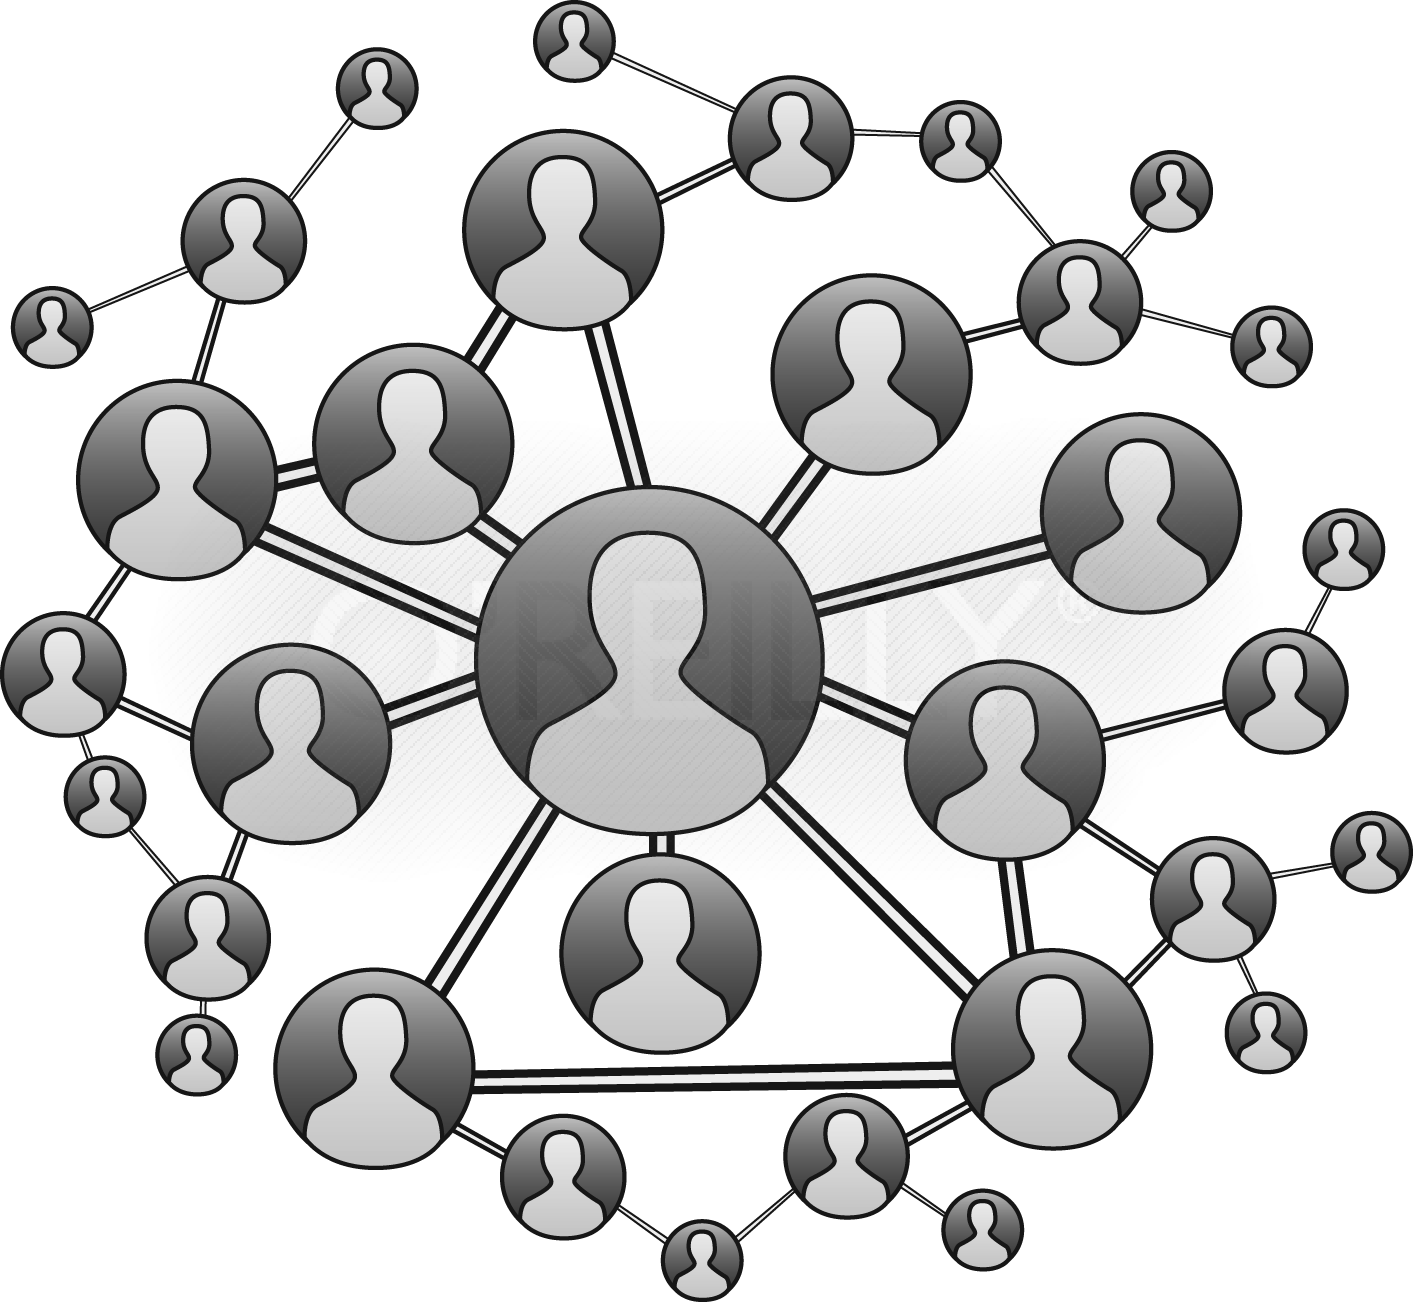
\includegraphics[height=0.35\textheight]{images/graph.png}}

\usetikzlibrary{graphs,arrows.meta}

\newcommand{\samplegraph}[1][1.2]{%
\begin{tikzpicture}[>=LaTeX,every node/.style={draw,circle,fill=diagramblue},scale=#1]
  \node (1) at (1,2)     {1};
  \node (2) at (3,2.2)   {2};
  \node (3) at (2,1)     {3};
  \node (4) at (0.8,0.2) {4};
  \node (5) at (2.5,0)   {5};
  \node (6) at (3.5,1.2)   {6};
  \graph {
    (1) -> {(2), (3)};
    (2) -> {(3), (6)};
    (3) -> {(4), (6)};
    (4) -> {(1), (5)};
    (5) -> (3);
    (6) -> (5);
  };
\end{tikzpicture}}

\newcommand{\emptygraph}{%
\begin{tikzpicture}[>=LaTeX,every node/.style={draw,circle,fill=diagramblue},scale=0.8]
  \node (1) at (1,2)     {1};
  \node (2) at (3,2.2)   {2};
  \node (3) at (0.8,0.2) {3};
  \node (4) at (2.5,0)   {4};
\end{tikzpicture}}

\newcommand{\fullgraph}{%
\begin{tikzpicture}[>=LaTeX,every node/.style={draw,circle,fill=diagramblue},scale=0.8]
  \node (1) at (1,2)     {1};
  \node (2) at (3,2.2)   {2};
  \node (3) at (0.8,0.2) {3};
  \node (4) at (2.5,0)   {4};
  \graph {
    (1) -> {(2), (3), (4)};
    (2) -> {(1), (3), (4)};
    (3) -> {(1), (2), (4)};
    (4) -> {(1), (2), (3)};
  };
\end{tikzpicture}}

\begin{document}

\begin{frame}
  \titlepage
\end{frame}

\section{Дефиниции}

\begin{frame}
  \frametitle{Дефиниция на граф}
  \begin{definition}[Граф]
    (Ориентиран) граф е наредена двойка $(V,E)$, където
    \begin{itemize}
    \item $V \neq \emptyset$ е произволно множество от \textbf{върхове}
    \item $E \subseteq V^2$ е множество от ребра
    \end{itemize}
  \end{definition}
  \pause
  Ако пренебрегнем реда на компонентите в двойките в $Е$, получаваме \textbf{неориентиран} граф.\\[1em]
  \begin{columns}[onlytextwidth]
    \begin{column}{0.5\textwidth}
      $E = \emptyset$ --- празен граф
      \emptygraph
    \end{column}
    \begin{column}{0.5\textwidth}
      $E = V^2$ --- пълен граф
      \fullgraph
    \end{column}
  \end{columns}
\end{frame}

\begin{frame}
  \frametitle{АТД: граф}
  Нелинейна структура, описваща обекти и връзките между тях.\\
  Операции:
  \begin{itemize}
  \item \tt{vertices()} --- списък на върховете
  \item \tt{successors()} --- списък на съседите на даден връх
  \item \tt{isEdge(a, b)} --- проверка за съществуване на ребро
  \item \tt{addVertex(a)} --- включване на връх
  \item \tt{removeVertex(a)} --- изключване на връх
  \item \tt{addEdge(a, b)} --- включване на ребро
  \item \tt{removeEdge(a, b)} --- изключване на ребро
  \end{itemize}
\end{frame}

\begin{frame}
  \frametitle{Етикети}
  Обектите и връзките в графа могат да бъдат свързани с етикети.\\[1em]
  \pause
  Нека е дадено множество $L$ от етикети.
  \begin{itemize}
  \item $v : V \rightarrow L$ --- етикети на върховете
  \item $e : E \rightarrow L$ --- етикети на ребрата
  \end{itemize}
\end{frame}

\begin{frame}
  \frametitle{Допълнителни дефиниции}
  \begin{itemize}[<+->]
  \item за $(u, v)\in E$, $u$ наричаме \textbf{предшественик}, а $v$ --- \textbf{наследник}
  \item $(u, u)$ наричаме \textbf{примка}
  \item $d^+(u) = |\{ v\;|\;(u, v) \in E\}|$ --- \textbf{положителна полустепен}
  \item $d^-(u) = |\{ u\;|\;(u, v) \in E\}|$ --- \textbf{отрицателна полустепен}
  \item $d(u) = d^+(u) + d^-(u)$ --- \textbf{степен на връх}
  \item \textbf{път} в граф наричаме редица $v_1, v_2, \ldots, v_n$, където $(v_i, v_{i+1}) \in E$
    \begin{itemize}
    \item ако $v_1 = v_n$, пътят е \textbf{цикъл}
    \item ако $v_i \neq v_j$ за $1 \leq i < j \leq n$, пътят е \textbf{ацикличен}
    \item ако $E = \{(v_i,v_{i+1})\;|\;1 \leq i < j \leq n\}$ и $|E| = n - 1$, пътят е \textbf{Ойлеров}
    \item ако $V = \{v_i\;|\;1 \leq i \leq n\}$ и $|V| = n$, пътят е \textbf{Хамилтонов}
    \end{itemize}
  \item граф е \textbf{цикличен}, ако в него има поне един цикъл
  \item граф е \textbf{(слабо) свързан}, ако $\forall a, b\in V$ има път от $a$ до $b$ (или от $b$ до $a$)
  \end{itemize}
\end{frame}

\section{Предствания на графи}

\begin{frame}<1-17>
  \frametitle{Матрица на съседство}
  \begin{columns}[onlytextwidth]
    \begin{column}{0.5\textwidth}
      \begin{equation*}
        A =
        \left(
          \begin{array}{*6c}
            0 & 1 & 1 & 0 & 0 & 0\\
            0 & 0 & 1 & 0 & 0 & 1\\
            0 & 0 & 0 & 1 & 0 & 1\\
            1 & 0 & 0 & 0 & 1 & 0\\
            0 & 0 & 1 & 0 & 0 & 0\\
            0 & 0 & 0 & 0 & 1 & 0
          \end{array}
          \right)
      \end{equation*}
    \end{column}
    \begin{column}{0.5\textwidth}
      \samplegraph
    \end{column}
  \end{columns}
  \pause
  \alt<-12>{
  \begin{itemize}[<+->]
  \item $A_{i,j} = 1 \leftrightarrow (i,j) \in E$
  \item памет --- \rvl{$O(|V|^2)$}
  \item \tt{successors} --- \rvl{$O(|V|)$}
  \item \tt{isEdge} --- \rvl{$O(1)$}
  \item \tt{addVertex, removeVertex} --- \rvl{$O(|V|)$}
  \item \tt{addEdge, removeEdge} --- \rvl{$O(1)$}
  \end{itemize}}{
  \begin{itemize}[<+(11)->]
  \item $A_{i,j} = 1 \leftrightarrow (v_i,v_j) \in E$
  \item $A^2_{i,j} > 0 \leftrightarrow \sum_{k=1}^n A_{i,k}A_{k,j} > 0 \leftrightarrow $ има път с дължина 2 от $v_i$ до $v_j$
  \item по индукция: $A^n_{i,j} > 0 \leftrightarrow $ има път с дължина $n$ от $v_i$ до $v_j$
  \item нещо повече: $A^n_{i,j}$ = броят на пътищата с дължина $n$ от $v_i$ до $v_j$
  \item ако $B = \sum_{k=1}^{|V|} A^k$, то $B_{i,j} > 0 \leftrightarrow$ има път от $v_i$ до $v_j$
  \end{itemize}}
\end{frame}

\begin{frame}<1-10>
  \frametitle{Матрица на инцидентност}
  \begin{equation*}
    A =
    \left(
      \begin{array}{*{10}c}
        -1 &  1 &  1 &  0 &  0 &  0 &  0 &  0 &  0 &  0\\
        0 & -1 &  0 &  0 &  0 &  1 &  0 &  1 &  0 &  0\\
        0 &  0 & -1 &  1 &  0 & -1 & -1 &  0 &  1 &  0\\
        1 &  0 &  0 & -1 &  1 &  0 &  0 &  0 &  0 &  0\\
        0 &  0 &  0 &  0 & -1 &  0 &  1 &  0 &  0 & -1\\
        0 &  0 &  0 &  0 &  0 &  0 &  0 & -1 & -1 &  1
      \end{array}
    \right)
  \end{equation*}
  \begin{columns}[onlytextwidth]
    \begin{column}{0.7\textwidth}
      \alt<1>{%
      \begin{itemize}
      \item $A_{i,j} = 1 \leftrightarrow \exists v \in V\, e_j = (v, v_i) \leftrightarrow e_j\text{ е \textbf{изходящо} ребро за }v_i$
      \item $A_{i,j} = -1 \leftrightarrow \exists v \in V\, e_j = (v_i, v) \leftrightarrow e_j\text{ е \textbf{входящо} ребро за }v_i$
      \end{itemize}
    }{%
      \begin{itemize}[<+->]
      \item памет --- \rvl{$O(|V||E|)$}
      \item \tt{successors} --- \rvl{$O(|E|+|V|)$}
      \item \tt{isEdge} --- \rvl{$O(|E|)$}
      \item \tt{addVertex, removeVertex} --- \rvl{$O(|E|)$}
      \item \tt{addEdge, removeEdge} --- \rvl{$O(|V|)$}
      \end{itemize}
    }
    \end{column}
    \begin{column}{0.3\textwidth}
      \samplegraph[1]
    \end{column}
  \end{columns}
\end{frame}

\begin{frame}
  \frametitle{Списък на наследници}
  \begin{columns}[onlytextwidth]
    \begin{column}{0.5\textwidth}
      \begin{equation*}
      D = \left\{
      \begin{array}{rcl}
        1 &\rightarrow& (2, 3)\\
        2 &\rightarrow& (3, 6)\\
        3 &\rightarrow& (4, 6)\\
        4 &\rightarrow& (1, 5)\\
        5 &\rightarrow& (3)\\
        6 &\rightarrow& (5)
      \end{array}\right\}
  \end{equation*}
    \end{column}
    \begin{column}{0.5\textwidth}
      \samplegraph
    \end{column}
  \end{columns}
  \begin{itemize}[<+->]
  \item $D_i = \{v\;|\;(v_i,v) \in E \}$
  \item памет --- \rvl{$O(|V|+|E|)$}
  \item \tt{successors} --- \rvl{$O(1)$}
  \item \tt{isEdge} --- \rvl{$O(|V|)$}
  \item \tt{addVertex} --- \rvl{$O(1)$}
  \item \tt{removeVertex} --- \rvl{$O(|E|)$}
  \item \tt{addEdge} --- \rvl{$O(1)$}
  \item \tt{removeEdge} --- \rvl{$O(|V|)$}
  \end{itemize}
\end{frame}

\begin{frame}
  \frametitle{Списък на инцидентност}
  \begin{columns}[onlytextwidth]
    \begin{column}{0.5\textwidth}
      \begin{equation*}
        \begin{array}{rll}
          E = ((1,2),&(2,3),&(3,6),\\
          (1,3),&(4,1),&(3,4),\\
          (5,3),&(6,5),&(4,5),\\
          (2,6))
        \end{array}
      \end{equation*}
    \end{column}
    \begin{column}{0.5\textwidth}
      \samplegraph
    \end{column}
  \end{columns}
  \begin{itemize}[<+->]
  \item памет --- \rvl{$O(|E|)$}
  \item \tt{successors} --- \rvl{$O(|E|)$}
  \item \tt{isEdge} --- \rvl{$O(|E|)$}
  \item \tt{addVertex} --- \rvl{$O(1)$}
  \item \tt{removeVertex} --- \rvl{$O(|E|)$}
  \item \tt{addEdge} --- \rvl{$O(1)$}
  \item \tt{removeEdge} --- \rvl{$O(|E|)$}
  \end{itemize}
\end{frame}
\end{document}
